\documentclass{lab_sheet}
\usepackage[hidelinks]{hyperref}
\newcommand\ddfrac[2]{\frac{\displaystyle #1}{\displaystyle #2}}


\begin{document}
    \titlePage{Time Division Multiplexing, Signal Reconstruction using Samples and Delta Modulation}{June 23, 2021}
    \pagenumbering{roman}
    \tableofcontents
    \clearpage
    \phantomsection
    \addcontentsline{toc}{section}{\bfseries{List of Figures}}
    \listoffigures
    \clearpage
    \phantomsection
    \addcontentsline{toc}{section}{\bfseries{Listings}}
    \lstlistoflistings
    \clearpage
    \pagenumbering{arabic}
    
\section{Objectives}
\begin{itemize}
    \item Perform time division multiplexing of two signals and recover the original signals.
    \item Perform reconstruction of a signal from its samples.
    \item Perform delta modulation and visualize the bit sequence for DM transmission.
\end{itemize}

\section{Background Theory}
\subsection{Time Division Multiplexing (TDM)}
TDM is the time interleaving of samples from different independent sources so that the information is transmitted serially over a single communication channel. This implementation of multiplexing enables the joint utilization of a common channel by a number of independent message signals without any interference.
\begin{figure}[H]
    \centering
    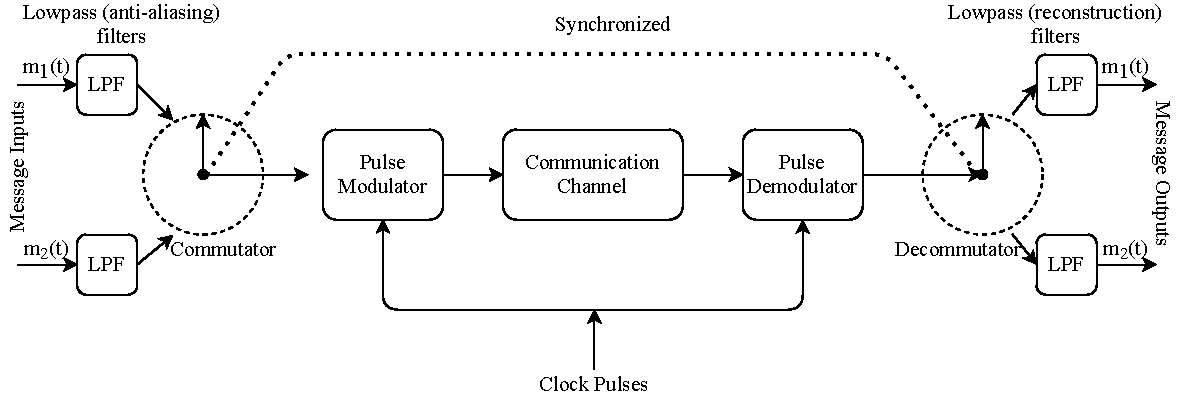
\includegraphics[width=\linewidth]{../Figures/tdm_block}
    \caption{Block diagram of TDM}
    \label{fig:tdm_block}
\end{figure}
Figure~\ref{fig:tdm_block} shows the block diagram for TDM, where each input message signal is band-limited with a lowpass pre-alias filter to remove the frequencies that are considered non-essential for transmission. Then the pre-alias filter outputs are applied to a commutator (implemented using electronic switching circuit) that takes a narrow sample of each of the N input message at the rate of $f_s$ that is higher than $2f_m$, where $fm$ is the cutoff frequency of pre-alias filter. It also performs the task of interleaving these N samples inside a sampling interval $T_s=\ddfrac{1}{f_s}$. The multiplexed signal is then applied in a pulse-amplitude modulator to transform the signal to a form suitable for transmission over the channel. At the receiver side, the signal is applied to a pulse-amplitude demodulator that produces short pulses which are distributed to appropriate lowpass reconstruction filters by the decommutator working in sync with the commutator.
\subsection{Sampling and signal reconstruction using samples}
Sampling is a process by which continuous time signals are converted into discrete time signal called samples. For a continuous time signal $s(t)$, the sampled discrete time signal $s[n]$ and sampling period of $T_s$, the sampling equation is given as,
\begin{equation}
    s[n]=s(nT_s)
\end{equation}
Sampling frequency $f_s=\ddfrac{1}{T_s}$ is used to denote sampling rate. For a continuous time signal $s(t)$ with $f_m$ as the highest frequency component, the Nyquist-Shannon theorem confines the sampling rate as,
\begin{equation}
    f_s>2f_m
    \label{eqn:sample_rate}
\end{equation}
Equation~\ref{eqn:sample_rate} must be satisfied to avoid aliasing of signal during sampling and for perfect reconstruction of the signal from its samples. The reconstruction of a signal using its samples is performed using a reconstruction filter, that is an ideal lowpass filter with cutoff at sampling frequency $f_s$. The passage of signal through this reconstruction filter corresponds to a convolution with the \textit{sinc} function in time domain. So a \textit{sinc} signal appears centered at each integer multiple of $T_s$ during reconstruction, which eventually settles to give the actual signal reconstructed using the samples, which is why this method of reconstruction is also known as ideal interpolation of samples.
\begin{figure}[H]
    \centering
    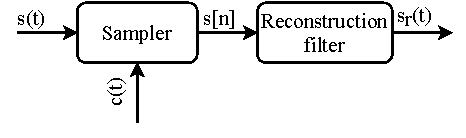
\includegraphics{../Figures/sample_block}
    \caption{Block diagram of sampling and reconstruction using samples}
    \label{fig:sample_block}
\end{figure}
\subsection{Delta modulation}
Delta modulation is a type of modulation where the sampling rate is much greater and the step-size after quantization is a smaller value $\Delta$. It is a simplified version of the Differential Pulse Code Modulation (DPCM). It uses a 1-bit quantizer and a delay circuit with two summer circuits which is why it is also known as 1-bit DPCM scheme. Only one binary bit per sample is transmitted.
\begin{figure}[H]
    \centering
    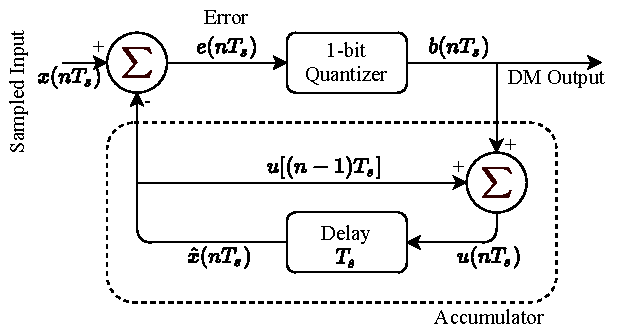
\includegraphics{../Figures/dm_block}
    \caption{Block diagram of delta modulation at transmitter}
    \label{fig:delta_block}
\end{figure}
Figure~\ref{fig:delta_block} shows the block diagram fro the delta modulation at transmitter. The summer in the accumulator adds quantizer output ($\pm \Delta$) with the previous sample approximation which gives present sample approximation as,
\begin{equation*}
    \begin{aligned}
        u(nT_s)&=u[(nT_s-T_s)]+ [\pm \Delta]\\
        u(nT_s)&=u[(n-1)T_s]+ b(nT_s)
    \end{aligned}
\end{equation*}
The previous sample approximation $u[(n-1)T_s]$ is restored by introducing delay $T_s$. The samples input signal $x(nT_s)$ and staircase approximated signal $\hat x(nT_s)$ are subtracted to get error signal $e(nT_s)$, depending on which the 1-bit quantizer gives either $+\Delta$ or $-\Delta$ as the step-size. For $+\Delta$ binary bit '$1$' is transmitted and for $-\Delta$ binary bit '$0$' is transmitted.
\section{Exercises}
\mysub{Time division multiplexing of two signals and recovery of signals}
\problem{Perform time division multiplexing of two signals and recover the original signals.}

\matlabcode{tdm}{Matlab script for time division multiplexing and recovery of original signals}
\begin{figure}[H]
    \centering
    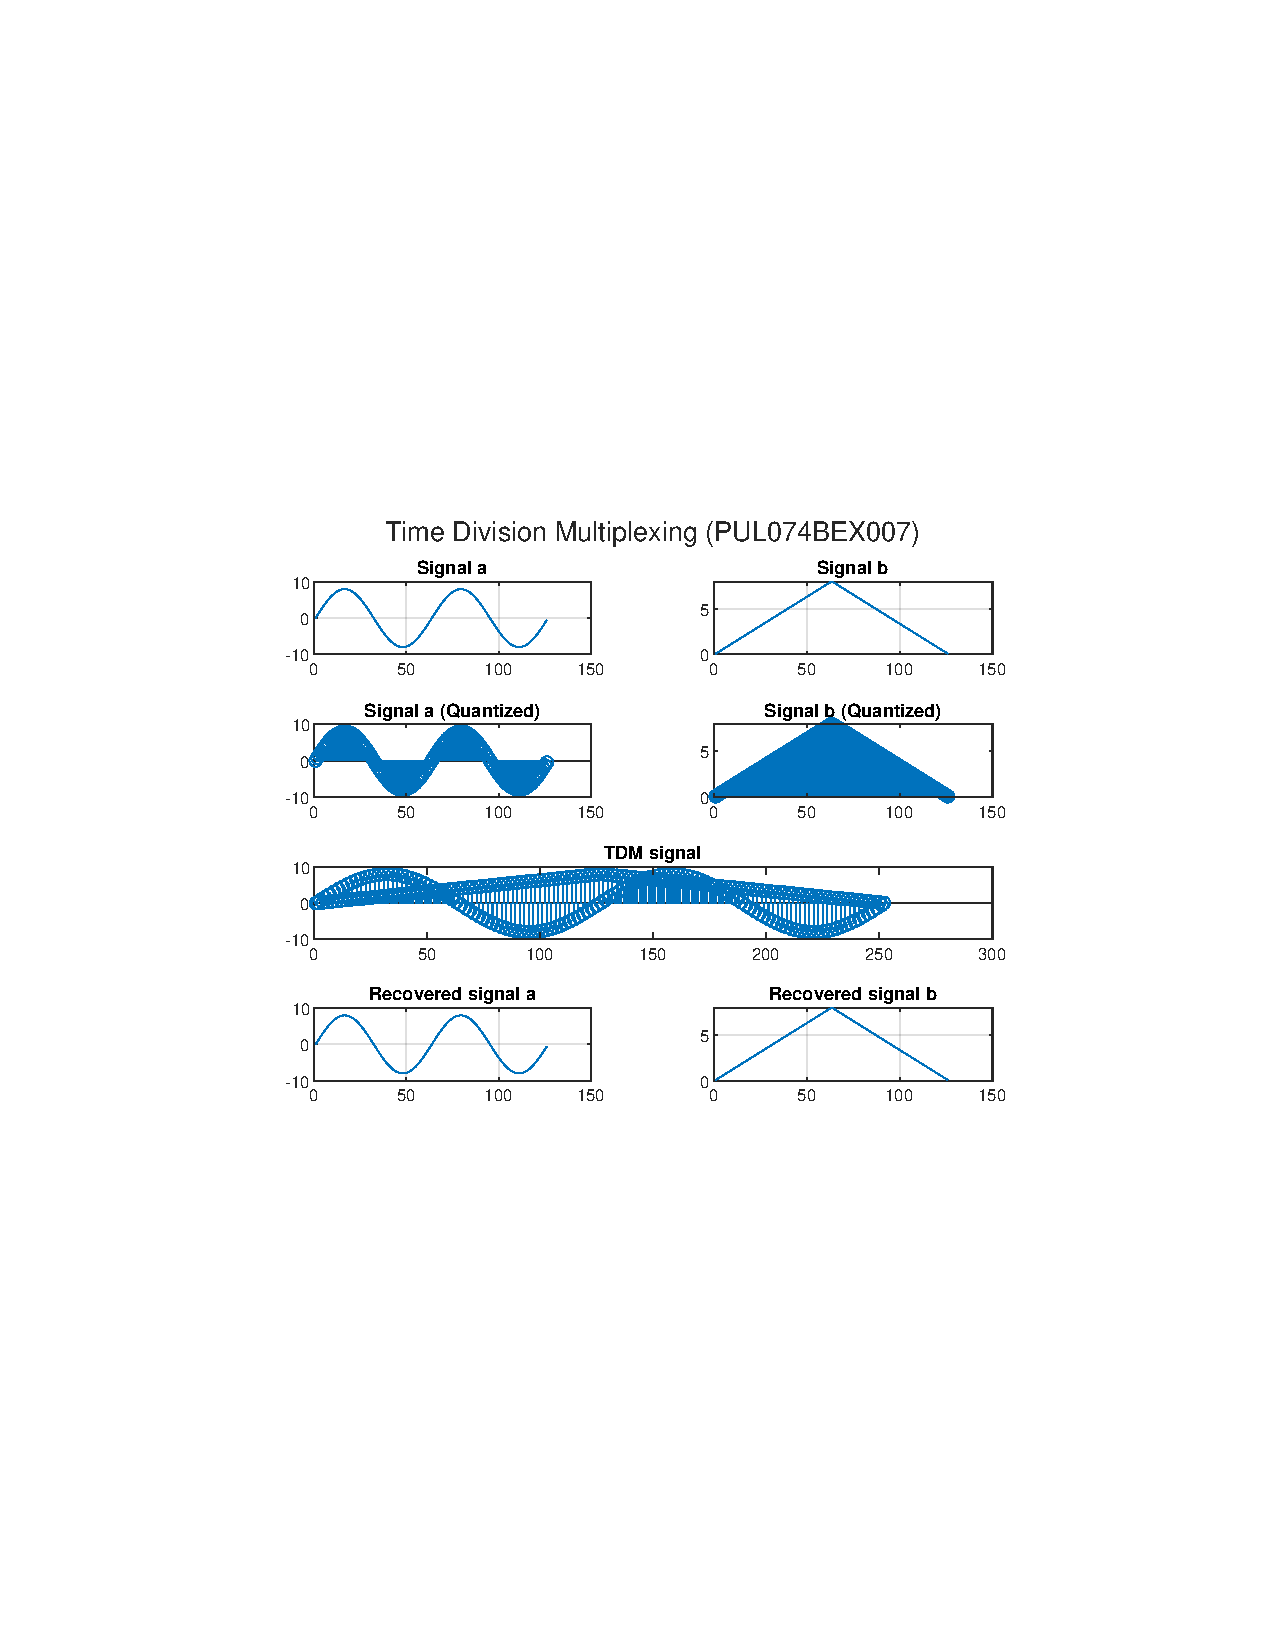
\includegraphics[width=0.8\linewidth]{../Figures/tdm}
    \caption{Time division multiplexing of two signals and recovered signals}
    \label{fig:tdm}
\end{figure}

\mysub{Reconstruction of a signal from its samples}
\problem{Perform reconstruction of a signal from its samples.}
\matlabcode{sampling}{Matlab script for sampling and reconstruction of a signal from its samples}

\begin{figure}[H]
    \centering
    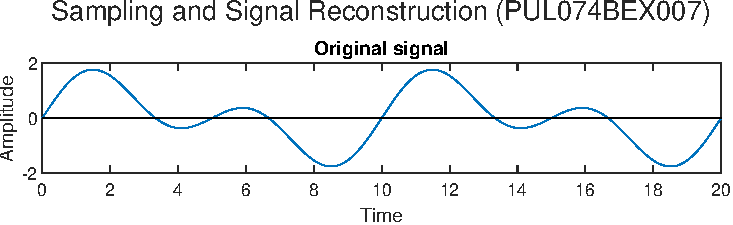
\includegraphics[width=0.8\linewidth]{../Figures/s_0}
    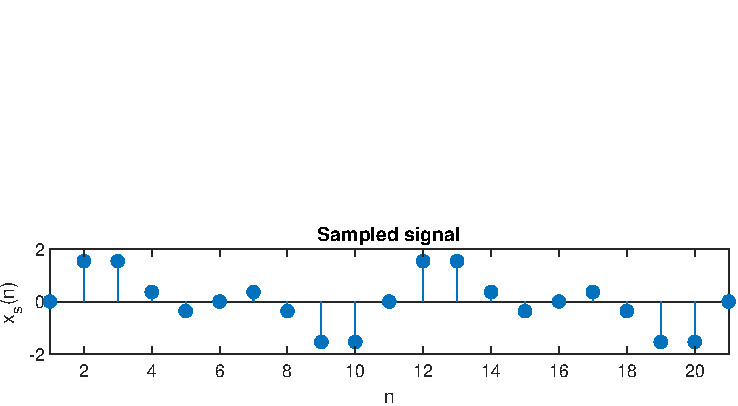
\includegraphics[width=0.8\linewidth]{../Figures/s_1}
    \caption{Reconstruction of a signal from its samples}
    \label{fig:sampling}
\end{figure}


\begin{figure}[H]
    \centering
    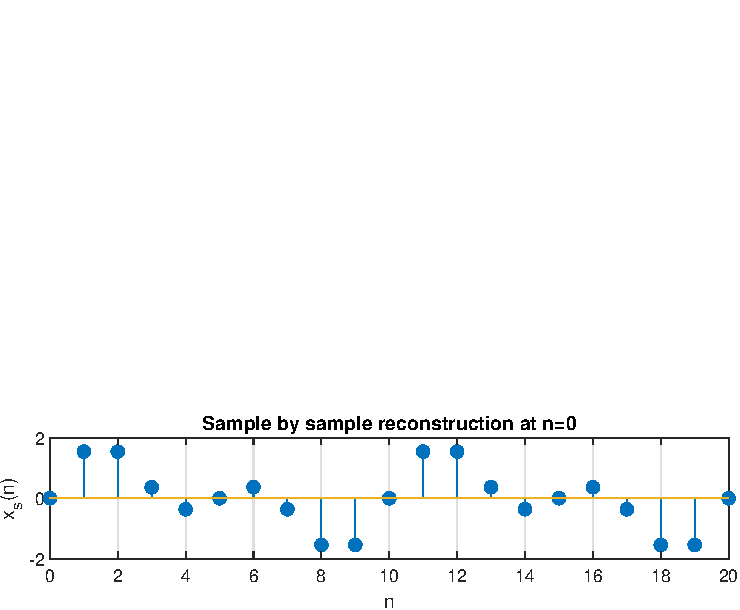
\includegraphics[width=0.8\linewidth]{../Figures/s_2}
    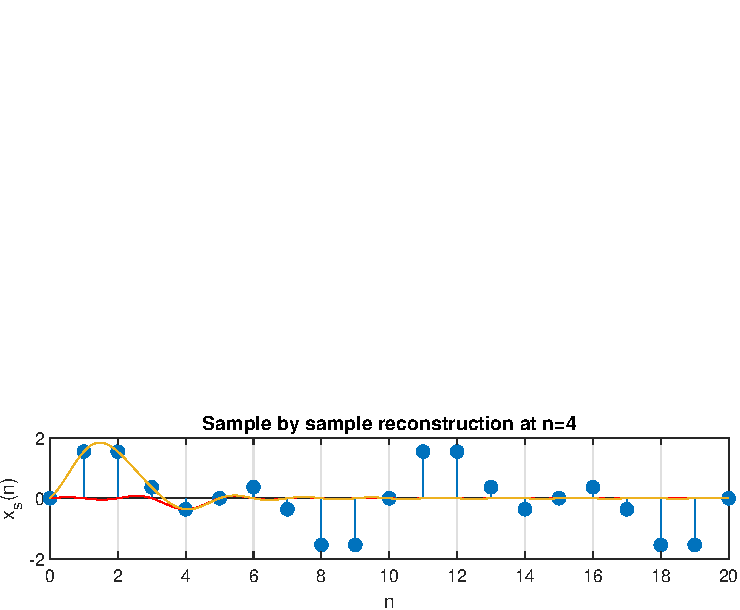
\includegraphics[width=0.8\linewidth]{../Figures/s_3}
    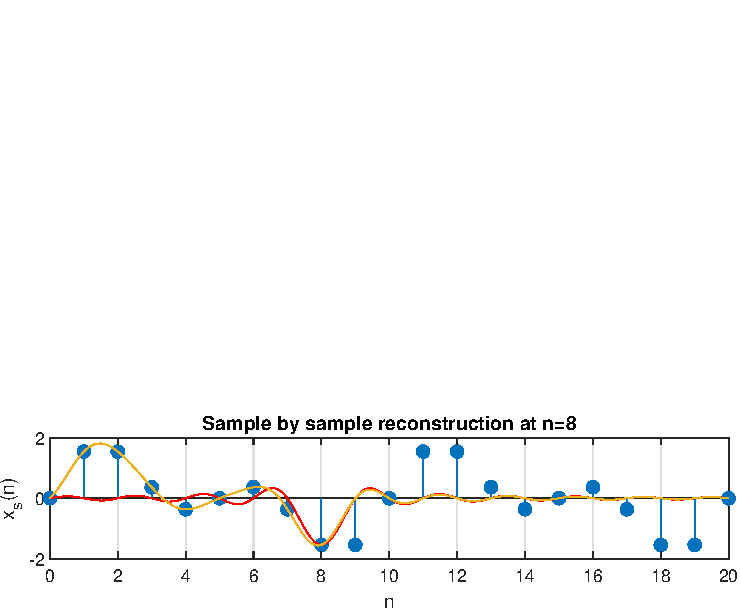
\includegraphics[width=0.8\linewidth]{../Figures/s_4}
    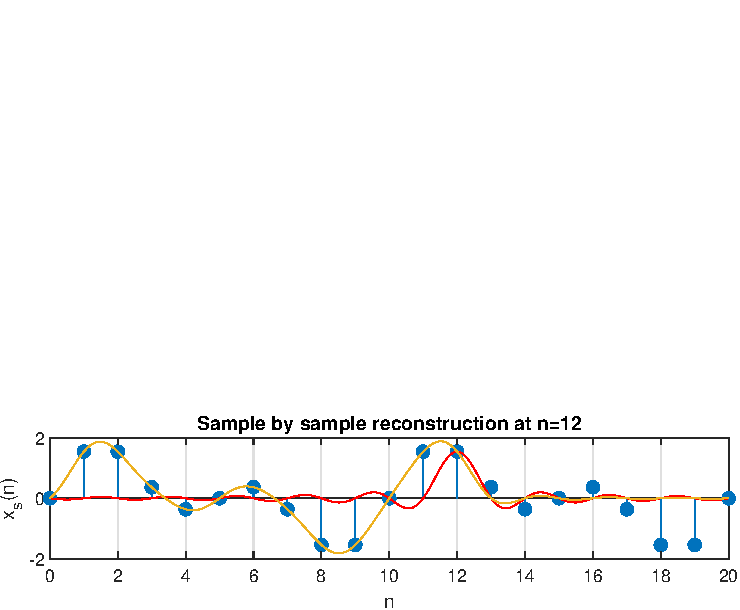
\includegraphics[width=0.8\linewidth]{../Figures/s_5}
    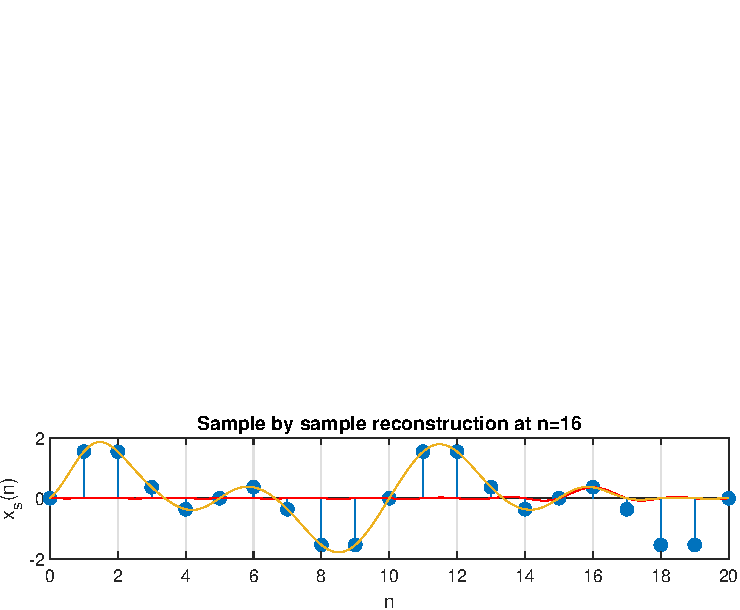
\includegraphics[width=0.8\linewidth]{../Figures/s_6}
    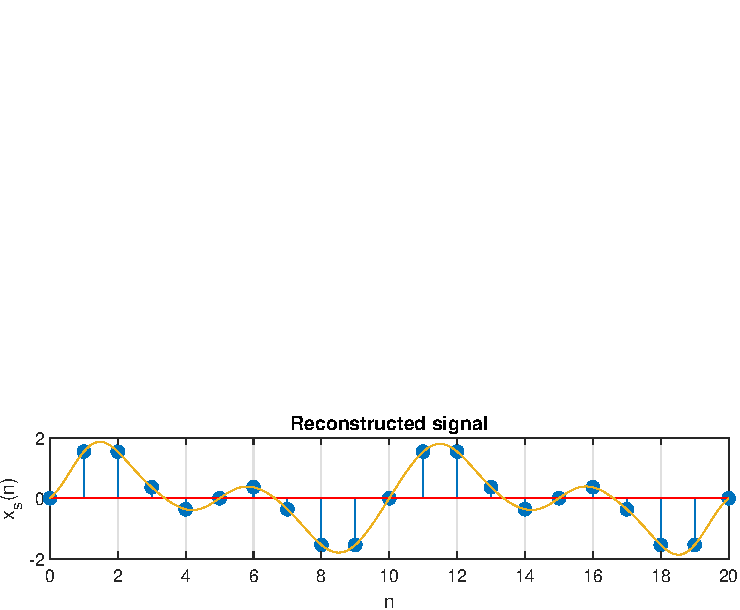
\includegraphics[width=0.8\linewidth]{../Figures/s_7}
    \caption*{Figure~\ref{fig:sampling}:~Reconstruction of a signal from its samples (continued)}
\end{figure}

\mysub{Delta modulation and bit sequence for delta modulation transmission}
\problem{Perform delta modulation and visualize the bit sequence for delta modulation transmission.}
\matlabcode{delta}{Matlab script for delta modulation and bit sequence for delta modulation transmission}
\begin{figure}[H]
    \centering
    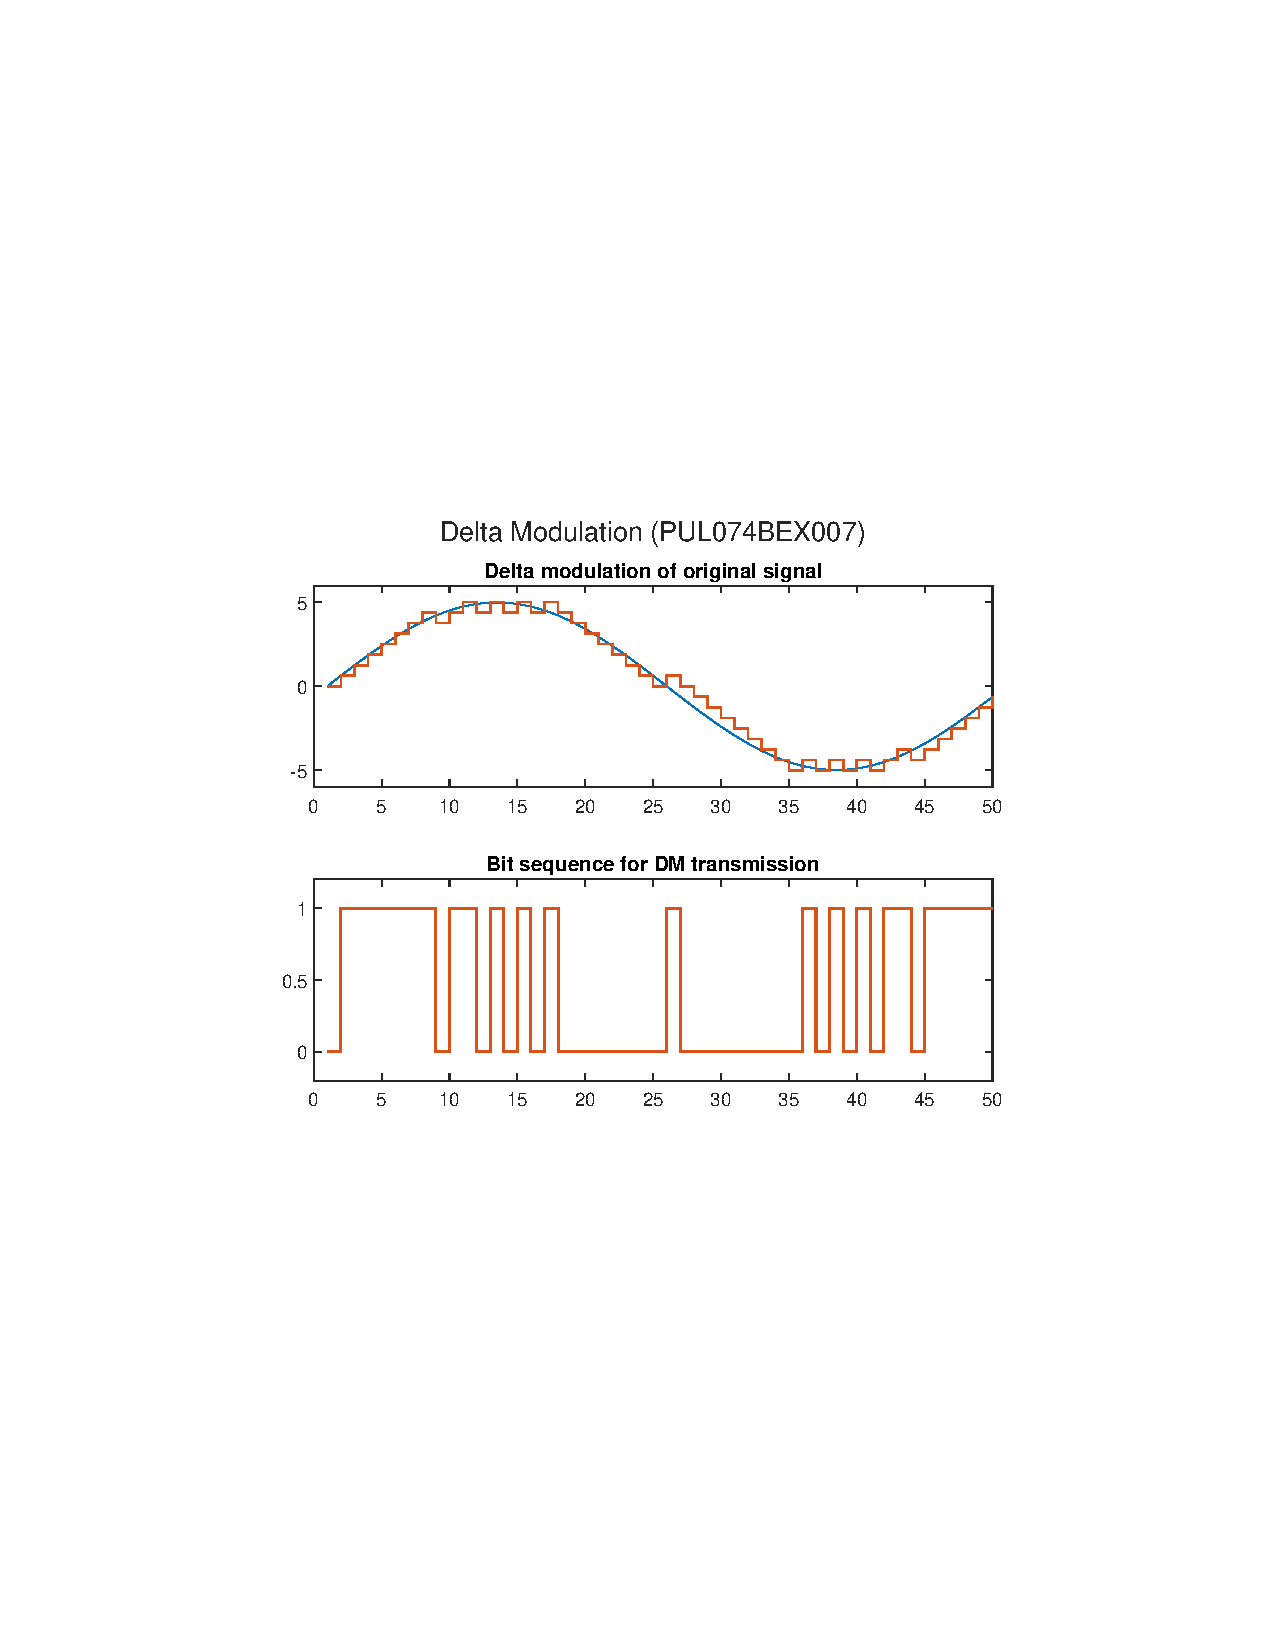
\includegraphics[width=0.8\linewidth]{../Figures/delta}
    \caption{Delta modulation and bit sequence for delta modulation transmission}
    \label{fig:delta}
\end{figure}

\section{Discussion and Conclusion}
The lab experiment dealt with the realization of time division multiplexing, signal reconstruction using samples and delta modulation.\\
TDM is a concept where multiple quantized signals are multiplexed in time and transmitted over the same channel as the multiplexed signal. On the receiving end a demultiplexer is used to recover the original signals. TDM allows low capacity communication channels to be used with little to no crosstalk while utilizing the full channel bandwidth.\\
Signal reconstruction using samples is a necessary topic of discussion since sampled signals can be used to recover the original signal with great accuracy. This is realized using a reconstruction filter which we coded in MATLAB. One thing to be noted is that sampling must suffice the Nyquist criteria so that signal integrity isn't lost on reconstruction.\\
Delta modulation is an AD/DA conversion technique mostly used for voice transmission where timely data delivery is prioritized over data quality. It requires less channel bandwidth than PCM since it generates only one bit per sample.\\
Hence the objectives of the lab experiment were fulfilled and the visualization of TDM, reconstruction of signals using samples and delta modulation were performed.
\end{document}
\end{document}